\documentclass[10pt,a4paper]{article}
\usepackage[utf8]{inputenc}
\usepackage{amsmath}
\newcommand{\RomanNumeralCaps}[1]
    {\MakeUppercase{\romannumeral #1}}
\usepackage{amsfonts}
\usepackage{amssymb}
\usepackage{float}
\usepackage{verbatim}
\usepackage{listings}
\usepackage{hyperref}

\usepackage{color} %red, green, blue, yellow, cyan, magenta, black, white
\definecolor{mygreen}{RGB}{28,172,0} % color values Red, Green, Blue
\definecolor{mylilas}{RGB}{170,55,241}
\usepackage{amsmath}
\usepackage{graphicx}
\graphicspath{{C:/Users/adria/Pictures/}} 
\author{Adrian Martinsen Kleven, Simon Schrader}
\title{INSERT TITLE!}

\lstset{
 	language =C++,   
    frame=tb, % draw a frame at the top and bottom of the code block
    tabsize=4, % tab space width
    showstringspaces=false, % don't mark spaces in strings
    numbers=left, % display line numbers on the left
    commentstyle=\color{green}, % comment color
    keywordstyle=\color{blue}, % keyword color
    stringstyle=\color{red} % string color
}

\begin{document}

\part*{--------Insert Title--------}
{\large By Simon Schrader (FYS4150) Adrian Kleven (FYS3150)}\\\\
\tableofcontents

\listoffigures
\listoftables

 
\clearpage
 
\section{Abstract}
Solving mathematical problems with the help of a computer has never been more relevant than nowadays and can be used for a broad range of problems. In this project, we compared three algorithms for solving a specific second-order differential equation, that we treated as a discretized linear algebra problem, numerically in terms of computational time and found that specializing our algorithms decreases computational time while retaining the same mathematical accuracy as the general algorithm. We also found that the accuracy is a function of step length, where  $h \approx 10^{-6}$ gives the result that is closest to the analytical solution of the equation we dealt with.
\section{Introduction}
\subsection{Purpose} 
The purpose of this report is to examine three different numerical algorithms for solving the one- dimensional Poisson equation with imposed Dirichelet boundary conditions. \\This equation can be rewritten as a set of linear equations and discretized for use in numerical approximations. Exploring the differences in computation time and relative error between the different algorithms will therefore also be a purpose of this report.\\\\
Another purpose is to become familiar with writing projects in C++, dealing with error handling and understanding the usefulness of implementing dynamic memory allocation of arrays and matrices in C++. Also, to practice presenting meaningful figures and tables as well as a comprehensive list of references.
\subsection{Approach}
For this specific set of equations, the general algorithm for Gaussian elimination of tridiagonal matrices can be specialised to a more appropriate algorithm for use on Toeplitz matrices. In addition, LU- decomposition will be explored in relation to the other algorithms.\\ By iterating the different algorithms with different step sizes and thereby, different number of iterations, the difference in computing time between algorithms can be illustrated more clearly. \\These methods are implemented in the C++ programming language and their results visualized using the Matplotlib python library.
\section{Methods}

As written in the Introduction, the aim is to solve a second-order differential equation of the form
$$\frac{d^2u(x)}{dx^2} = -g(x).$$

Using the formula 3.4 in [1], this equation can be discretized to 
$$\frac{u_{i-1}-2u_{i}+u_{i+1}}{h^2} = g_{i}$$
where $u_{i}$ and $g_{i}$ stand for $u(x_{i})$ and $g(x_{i})$, respectively, and $x_{i}=i*h$, where we discretize the problem in $n$ values and  $h=\frac{1}{n+1}$, and $i  \in  \mathbb{Z}$.
In our case, we know that $g(x)$, that is, the second derivative, is given by the equation $g(x) = 100e^{-10x}$. Dirichlet boundary conditions apply, where $u(0)=u(1)=0$.
This problem can thus represented as a matrix:
\[
    \mathbf{A} = \begin{bmatrix}
                           2& -1& 0 &\dots   & \dots &0 \\
                           -1 & 2 & -1 &0 &\dots &\dots \\
                           0&-1 &2 & -1 & 0 & \dots \\
                           & \dots   & \dots &\dots   &\dots & \dots \\
                           0&\dots   &  &-1 &2& -1 \\
                           0&\dots    &  & 0  &-1 & 2 \\
                      \end{bmatrix}\begin{bmatrix}
                           u_1\\
                           u_2\\
                           \dots \\
                          \dots  \\
                          \dots \\
                           u_n\\
                      \end{bmatrix}
  =h^2
\begin{bmatrix}
                           {g}_1\\
                           {g}_2\\
                           \dots \\
                           \dots \\
                          \dots \\
                           {g}_n\\
                      \end{bmatrix}.
\]
when $u_{0}=u_{n+1}=0$, as in our case. In order to shorten notation, $g_i*h^2$ is simply written as  $g_i$ from now on.
To solve this problem, we applied 3 different approaches: Gaussian elimination of a general tridiagonal matrix, Gaussian elimination using an improved algorithm for this specific tridiagonal Toeplitz matrix, and LU decomposition of a general matrix. The accuracy of our solutions can be determined by calculating the relative error, which we can calculate because we know the analytical solution given by 
$$u(x)=1-(1-e^{-10})x-e^{-10x}$$
\subsection{Gaussian elimination of a tridiagonal matrix} 
The task is to solve an equation in this general form for the vector $\mathbf{u}$ :\\
\[
    \mathbf{A} = \begin{bmatrix}
                           b_1& c_1 & 0 &\dots   & \dots &\dots \\
                           a_1 & b_2 & c_2 &\dots &\dots &\dots \\
                           & a_2 & b_3 & c_3 & \dots & \dots \\
                           & \dots   & \dots &\dots   &\dots & \dots \\
                           &   &  &a_{n-2}  &b_{n-1}& c_{n-1} \\
                           &    &  &   &a_{n-1} & b_n \\
                      \end{bmatrix}\begin{bmatrix}
                           u_1\\
                           u_2\\
                           \dots \\
                          \dots  \\
                          \dots \\
                           u_n\\
                      \end{bmatrix}
  =\begin{bmatrix}
                           {g}_1\\
                           {g}_2\\
                           \dots \\
                           \dots \\
                          \dots \\
                           {g}_n\\
                      \end{bmatrix}.
\]
Where $a_n$,$b_n$, and $c_n$ are real numbers and the diagonal elements are nonzero.\\
This can be done by applying the normal Gaussian elimination. The algorithm to do so is as follows:
$$\tilde{a}_i = 0$$
$$\tilde{b}_i=b_i-\frac{a_i}{\tilde{b}_{i-1}} c_{i-1}$$
$$\tilde{g}_i=g_i-\frac{a_i}{\tilde{b}_{i-1}} \tilde{g}_{i-1}$$
Leaving us with the following system:
\[
    \mathbf{A} = \begin{bmatrix}
                           b_1& c_1 & 0 &\dots   & \dots &\dots \\
                           0& \tilde{b}_{2} & c_2 &\dots &\dots &\dots \\
                           & 0 & \tilde{b}_{3} & c_3 & \dots & \dots \\
                           & \dots   & \dots &\dots   &\dots & \dots \\
                           &   &  & 0  &\tilde{b}_{n-1}& c_{n-1} \\
		      &    &  &   &0 &\tilde{b}_n  \\
                      \end{bmatrix}\begin{bmatrix}
                           u_1\\
                           u_2\\
                           \dots \\
                          \dots  \\
                          \dots \\
                           u_n\\
                      \end{bmatrix}
  =\begin{bmatrix}
                           g_1\\
                           \tilde{g}_2\\
                           \dots \\
                           \dots \\
                          \dots \\
                           \tilde{g}_n\\
                      \end{bmatrix}.
\]
The solutions can then be found by backward substitution: 
$$u_n = \frac{\tilde{g}_n}{\tilde{b}_n}$$
$$u_{i-1} = \frac{\tilde{g}_{i-1}-c_{i-1} u_i}{\tilde{b}_{i-1}}$$
When calculating the step $\frac{a_i}{\tilde{b}_{i-1}}$ only once, we are left with approximately $8n$ floating point operations.
\subsection{Gaussian elimination of the specific tridiagonal Toeplitz matrix}

Because $c_i=a_i=-1$, the previously described algorithm used for the specific matrix  to solve the second derivative problem can be improved. It can be shown that 
$$\tilde{b}_i=\frac{i+1}{i}$$
This very step can be very efficiently precalculated, thus it will not go into the calculation of the number of floating point operations. The rest of the algorithm goes as follows.
$$\tilde{g}_i=g_i+\frac{\tilde{g}_{i-1}}{\tilde{b}_{i-1}} $$
Followed by backward substitution:
$$u_n = \frac{\tilde{g}_n}{\tilde{b}_n}$$
$$u_{i-1} = \frac{\tilde{g}_{i-1}+u_i}{\tilde{b}_{i-1}}$$
The number of floating point operations is thus approximately $4n$.\\

\subsection{LU-Decomposition}
Given a non- degenerate matrix $ M \in \mathbb{R} ^{n\times n}  $ where $n \in \mathbb{N}$\\$M$ can be factored into an upper- and a lower- triangular matrix.
$$
\textbf{A} =\textbf{LU} =
\begin{bmatrix}
a_{11} & a_{12} & a_{13} & a_{14} \\
a_{21} & a_{22} & a_{23} & a_{24} \\
a_{31} & a_{32} & a_{33} & a_{34} \\
a_{41} & a_{42} & a_{43} & a_{44} \\
\end{bmatrix}=
\begin{bmatrix}



1 & 0 & 0 & 0 \\
l_{21} & 1 & 0 & 0 \\
l_{31} & l_{32} & 1 & 0 \\
l_{41} & l_{42} & l_{43} & 1 \\
\end{bmatrix}
\begin{bmatrix}
u_{11} & u_{12} & u_{13} & u_{14} \\
0 & u_{22} & u_{23} & u_{24} \\
0 & 0 & u_{33} & u_{34} \\
0 & 0 & 0 & u_{44} \\
\end{bmatrix}
$$
Using the properties of the matrix we can arrive at the expressions for each of the matrix elements $l_{ij}$ and  $u_{ij}$ expressed in terms of the matrix elements $a_{ij}$. Since the matrix elements of A are known and the diagonal elements of the lower- triangular matrix $l_{ii}$ are 1, we can arrive at algorithm know as Doolittle's algorithm for LU- decomposition.\\\\
\begin{equation}
u_{1j} = a_{1j}
\end{equation}
For elements $u_{ij}, i= 2,...,,j-1$
\begin{equation}
u_{ij} = a_{ij} - \sum_{k=1}^{i-1}l_{ik}u_{kj}
\end{equation}
\begin{equation}
u_{jj} = a_{jj} - \sum_{k=1}^{j-1}l_{jk}u_{kj}
\end{equation}
\begin{equation}
l_{ij} = \frac{1}{u_{jj}} \Bigg( a_{ij} - \sum_{k=1}^{i-1}l_{ik}u_{kj} \Bigg)
\end{equation}
Once the matrix is expressed as the product of the lower- and upper- triangular matrices, the linear system of equations is solved in two parts. Using the inverse of a matrix and forward substitution.
$$
\textbf{Ax} =\textbf{LUx} = \textbf{w}
$$
$$
\textbf{Ux} =\textbf{y}
$$
$$
\textbf{Ly} =\textbf{w}
$$
Since the matrix $L$ is non- degenerate, $\textbf{y}$ can be written in terms of the inverse of $\textbf{L}$.\\
$$
\textbf{y} =\textbf{ L}^{\textbf{-1}}\textbf{w}
$$
With $y$, $x$ can be obtained by $\textbf{Ux} =\textbf{y}$, and our linear system of equations is solved.\\\\By using the equations 2 through 4, it can be found that the total number of floating point operations for the LU- factorization is approximately $\frac{2}{3}n^3$, according to [1] .
\subsection{C++ Implementation}
\subsubsection{General tridiagonal matrix}
The code where the algorithms were implemented, can be found here: \\
The core of the general triangular Gaussian elimination algorithm is given by the following C++ code snippet:
\begin{lstlisting}[caption=Code for solving the general triangular matrix]
void solve(double *a,double *b,double *c,
		   double *deriv,int n,double *solutions){
  
  double precalc;
  for(int i=1;i<n;i++){
    precalc=a[i+1]/b[i];
    
    //b[i+1]=b[i+1]-a[i+1]*c[i]/b[i];
    b[i+1]=b[i+1]-precalc*c[i]; 
    deriv[i+1]=deriv[i+1]-precalc*deriv[i];
  }
  solutions[n]=deriv[n]/b[n];
  delete [] a; // A not needed anymore (set to 0 anyways)
  for(int i=n-1;i>=1;i--){
    solutions[i]=(deriv[i]-c[i]*solutions[i+1])/b[i];
  }
  //c and b and deriv are not needed anymore
  delete [] c; delete [] b; delete [] deriv; 
}
\end{lstlisting}
Here $a$, and $b$ are arrays of length $n+1$ (the 0th value remains unused), $c$ is an array of length $n$, and $deriv$ (the discretized second derivative multiplied with $h^2$) is an array of length $n+2$. $n$ is the size of the $ n\cdot n$ matrix. $solutions$ is an array of length $n+2$ and the array that is changed, while the space for the other arrays is freed.\\\\
\subsubsection{Tridiagonal Toeplitz matrix}
The core of the algorithm for solving the specific matrix encountered is given by the following C++ code sniplet:
\begin{lstlisting}[caption=Code for solving the specific triangular matrix]
void improvedSolve(double *deriv,double *b,
				   int n, double *solutions){
  for(int i=2;i<=n;i++){
    deriv[i]=deriv[i]+deriv[i-1]/b[i-1];
  }
  solutions[n]=deriv[n]/b[n];
  for(int i=n-1;i>=1;i--){
    solutions[i]=(deriv[i]+solutions[i+1])/b[i];
  }
  delete [] b; delete [] deriv;
}
\end{lstlisting}
Here, $deriv$ (the discretized second derivative multiplied with $h^2$) is an array of length $n+2$, b is an array of length $n+1$ (0th element is ommitted) and already filled with the changed values.  $n$ is the size of the $n\cdot n$ matrix. $solutions$ is an array of length $n+2$ and the array that is changed, while the space for the other arrays is freed.\\
In all cases, the results were verified by comparing the calculated result using the algorithms to the analytical solution, which exists for our given problem. The intermediate matrices were printed to the terminal to assure that the algorithms were, in fact, implemented correctly. 
\subsubsection{LU- decomposition}

the lib- library functions \emph{ludcmp} and  \emph{lubksb} are used to implement the LU- decomposition and solver into our program.
\begin{lstlisting}[caption=Calling the inbuilt lib.cpp functions "ludcmp" and "lubksb" on the matrix A]
int          i,j, *indx;
double       d, *col, **y;
  // allocate space in memory
  indx = new int[n];
  col  = new double[n];
  start=clock();
  ludcmp(A,n,indx,&d);
  lubksb(A,n,indx,deriv);
  finish=clock();
  deleteNNMatrix(A,n);
\end{lstlisting}
Where n is the dimension of the matrix A, indx is an array recording the row permutations, d is a number determining whether the number of row interchanges is even or odd. Deriv outputs as the solution to the linear set of equations. This program is repeated for n- by n- matrices of size n =10,100 and 1000.

\subsection{Accuracy}
For all algorithms, the results were verified by comparing the calculated result using the algorithms to the analytical solution, which exists for our given problem. For each algorithm, for each $x_i$, both the analytical result and the result using the algorithm were written to a .txt file. The analytical solution as well as the approximate solutions can be plotted to inspect if the algorithm is generally right, while looking at the relative error as a function of the step length $h$ is a more reliable and exact way to see how accurate the solution is. 
\section{Results}

\subsection{Precision}

\begin{figure}[H]
	\includegraphics[width =1.2\textwidth]{approx_vs_analytical.png}
	\caption[Precision of the generalized algorithm]{The discretized solution for different values of n compared to the analytical solution using Gaussian substitution of a general tridiagonal matrix}
\end{figure}


Here, we see that discretizing with only $n=100$ steps already yields very usable results in the sense that the dimension of result is correct.
\begin{figure}[H]
	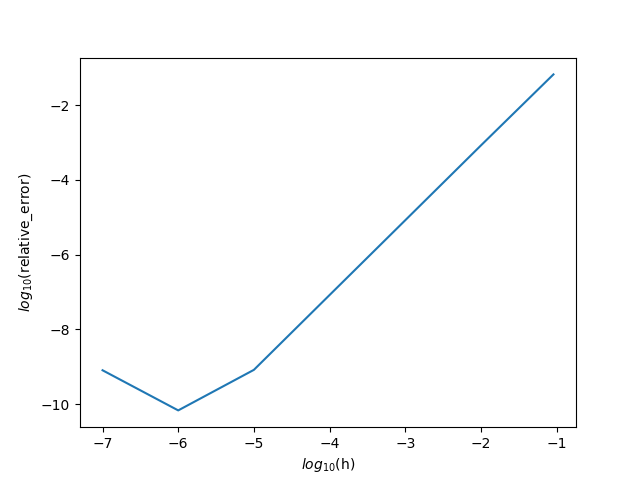
\includegraphics[width =1.2\textwidth]{error.png}
	\caption[Relative error of specialized algorithm]{Logarithm of maximum relative error of specialized algorithm as a function of logarithm of step length}
	\label{Figure 3}
\end{figure}
One can clearly see how the logarithm of the error decreases almost linearly as a function of the logarithm of h until $log_{10}(h)$, where the error starts increasing again. This is expected. The (probable) leading term of the mathematical error in the second derivative is given by $$\epsilon_{approx}=\frac{{f_0}^{(4)}}{12}h^2,$$ so in principle, increasing n (thus decreasing h) will reduce the error and only time use can hinder us in decreasing the error to zero. However, due to the nature of loss in numerical precision in double precision numbers in C++, we get a maximum in accuracy at $n \approx 10^6$.  This is probably because very small differences between $g_i$ and $g_{i+1}$
 are not correctly represented anymore and errors start accumulating.
\subsection{Time expenditure}
The number of floating point operations used by an algorithm is only indicative of the time spent by a computer. Fetching from and writing to memory contribute to the total time spent computing. So, in order to compare the efficiencies of these algorithms, it's useful to run and time the different programs in order to assess their performance compared to each other.\\To do this, the different algorithms where timed and averaged over 31 simulations each using the inbuilt \emph{time.h} functions. The results are shown below in Figure \ref{Figure 2}.
\begin{center}
\begin{figure}[H]
\includegraphics[width =1.2\textwidth]{IMG1217.jpg} \label{Elapsed time comparison}
	\caption[Comparing elapsed time]{Average elapsed time as measured by averaging 31 simulations of each algorithm. Plotted on a logarithmic scale.}
	\label{Figure 2}
\end{figure}
\end{center}
As seen from this figure, the time spent by the LU- decomposition of a general matrix rises exceptionally quickly as the matrix grows in size compared to the two other algorithms.\\\\It is also of interest to compare the general and specialized approaches to see what improvements were made. In this case, the number of floating point operations halved when switching from a general to a specialized algorithm. Again, taking the average of 31 simulations of each algorithm, then plotting their ratio as a function of the matrix size. This is shown below in figure \ref{Figure 3}
\begin{center}
\begin{figure}[H]
	\includegraphics[width =1.2\textwidth]{IMG1218.jpg}
	\caption[Comparing general and specialized (elapsed time)]{The ratio of time- expenditure between the specialized and general algorithm as a function of the size of matrix plotted logarithmically}
	\label{Figure 3}
\end{figure}
\end{center}
The ratio quickly drops from around 0.95 to around 0.75 as the size of the matrix grows. This is significantly higher than an estimate based solely on floating point operations, according to which the ratio should be $\approx0.5
$. This suggests that other factors have a significant impact on the results.

\section{Conclusion}
The results that were found in this project agreed with our expectations. When we varied the matrix size $n$, we expected to see a decrease in the error due to a reduced mathematical error until a given point from which it would start raising again due to roundoff errors, and found that this point is at around $n \approx 10^6$. We also wanted to see how specializing an algorithm can lead to increased efficiency while yielding the same results, and we found that the expense of formulating and implementing specialized algorithms, like the Thomas algorithm, are absolutely worth it, considering how personal computers are unable to solve a general matrix of size $10^5\times10^5$ or bigger both in terms of memory use and computational time - storing $10^{10}
$ double precision variables, 8 bytes each, takes approximately 80 gigabytes of Random Access Memory, which is five to ten times more than modern computers have. We found that the number of floating point operations is roughly proportional to the time use of our program, and that reducing the number of FLOPS from 8n to 4n reduced the computational speed by over 25\% for matrices of size $3\times 3$ and greater. Even though these findings were of mathematical nature, they are very relevant for problems in natural sciences, were time use and accuracy are of uttermost importance. We have developed a set of tools that can be used for a broad range of purposes, not just this project.
\section{Appendix}
\subsection{Proof that $\tilde{b}_i=\frac{i+1}{i}$ in the improved algorithm}
By calculation by hand, it can be shown that  $\tilde{b}_1=\frac{2}{1}$,  $\tilde{b}_2=\frac{3}{2}$.\\
This gives the impression that  $\tilde{b}_i=\frac{i+1}{i}$.
Inserting this in the general algorithm for Gauss elimination, we can perform a proof by induction and get that
 $$\tilde{b}_{i+1}=2-\frac{1}{\tilde{b}_{i}}=2-\frac{i}{i+1}=\frac{i+2}{i+1} \blacksquare$$
\subsection{List of programs}
All programs can be found on \url{https://github.com/adrian2208/FYS3150_collab}
\begin{enumerate}
\item b.cpp - Solves the problem using Gaussian elimination of any tridiangular matrix
\item c.cpp - Solves the problem using Gaussian elimination of specific tridiangular matrix decomposition
\item e.cpp - Solves the problem using LU decomposition, writes to file
\item vecop.cpp and vecop.hpp - Library files with actual solving functions
\item d.py creates the file log\_err\_c.txt with maximum relative error.
\item plot\_from\_output.py $log_{10}(h)$
\item plot\_times.py - plots time use from time\_
info.txt
\item plot\_h.py - plots $log_{10}(h)$ against $log_{10}(rel_error)$
\item run\_everything.py - runs b.cpp, c.cpp and e.cpp 30 times without writing to file, then once with writing to file, for varying n
\end{enumerate}
\subsection{Tables}
\begin{table}[H]
\caption[Relative error of specialized algorithm]{Logarithm of maximum relative error of specialized algorithm as a function of logarithm of step length}
\begin{tabular}{ll}
$log_{10}(h)$ &  $log_{10}(max_{\epsilon_i})$ \\
 -1.041 & -1.180 \\
 -2.004 & -3.088 \\
 -3.000 & -5.080 \\
 -4.000 & -7.079 \\
 -5.000 & -9.079 \\
 -6.000 & -10.163 \\
 -7.000 & -9.090 

\end{tabular}
\end{table}

\section{References}
[1] Morten Hjort-Jensen \textit{Computational Physics: Lecture Notes Fall 2015}



\begin{comment}

$$
\begin{bmatrix}
0 & 0 & 0 & 0 \\
0 & 0 & 0 & 0 \\
0 & 0 & 0 & 0 \\
0 & 0 & 0 & 0 \\
\end{bmatrix}
$$

\begin{lstlisting}[caption=insert caption]
for (unsigned int i = 0; i<100;i++{
}
\end{lstlisting}

\begin{figure}[h]
\includegraphics[width=8cm]{}
\caption{include caption}
\end{figure}

\end{comment}

\end{document}